\documentclass[10pt,report,compsoc, onecolumn]{./class/IEEEtran}
\hyphenation{op-tical net-works semi-conduc-tor}
\usepackage{graphicx}
\usepackage{multirow}
\usepackage[hyphens]{url}	% allow URL breal
\usepackage{hyperref}	% links from the reference to the source
\usepackage{listings}	% for code snippets
\usepackage{pgfplots} 	% graphics
\usepackage{flushend}	% balance columns at the end of the paper
\usepackage{caption}
\usepackage{subcaption}






\begin{document}
\title{Report: Analysing resource allocation for a distributed monitoring application}

\author{\IEEEauthorblockN{
Bogdan-Constantin Irimie\IEEEauthorrefmark{1}\IEEEauthorrefmark{2}}
\IEEEauthorblockA{ 
	\IEEEauthorrefmark{1}Institute e-Austria Timisoara, Romania\\
	\IEEEauthorrefmark{2}Department of Computer Science, West University of Timisoara, Romania}
}


\maketitle

\begin{abstract}
In a cloud environment monitoring applications should be able to scale in order to satisfy the monitoring requirements offering good quality of service and efficient resource utilization. In order for this scaling to be possible, monitoring applications should be built from the ground up with this goal in mind and mechanism for auto scaling should be implemented in order to provide a fast adaptation time. This report describes the work that has been done in order to enhance a monitoring system with automatic resource allocation capabilities. The work describes possible architectures with their advantages and drawbacks and implementations with their technical challenges.
\end{abstract}

\section*{Introduction}

Monitoring plays an important role in todays offerings of cloud computing because it enables cloud providers and consumers to check if the quality of service they have agreed upon is satisfied, additionally monitoring can be used to verify that a certain level of security is enabled. 

Resources in the cloud can be provisioned and released with ease, in a short period of time, and monitoring systems should be able to scale just as fast in order to adapt to the new monitoring requirements. In order to adapt, the monitoring systems should relay on a resource allocation mechanism that can take into account the architectures of the monitoring systems and provide strategies for resource allocation. The architecture of the monitoring systems is very important because it dictates the means of obtaining scalability, some systems having architectures that allow scaling because they providing decoupled systems where each component can be scaled independently,very similar to the micro-services architecture \footnote{http://microservices.io/patterns/microservices.html}, while other systems are build on a monolithic architecture making scaling more challenging and in some cases even impossible.

In this report we will focus on a monitoring system that implements a pipe and filter architecture allowing independent scaling, via replication, for all components, and thus providing fault tolerance and parallel execution of jobs.

\section{Analyzing the system and it's architecture}
The architecture of the system is important because it dictates the means by which scalability can be obtained. In Fig. \ref{fig:systemArchitecture} the architecture of the system is presented, this architecture being an extension of [cite paper from SYNASC]. The system is composed of 7 components: FrontEnd, Scanner, Converter, Presenter, Remediator, a document database and a message queue. The first five components send messages using the queue and are completely decoupled from one another, from each component perspective the system is only compose of itself and one or more message queues. This decoupling provides grate opportunity for replication and scalability.

\begin{figure}[ht]
\centering
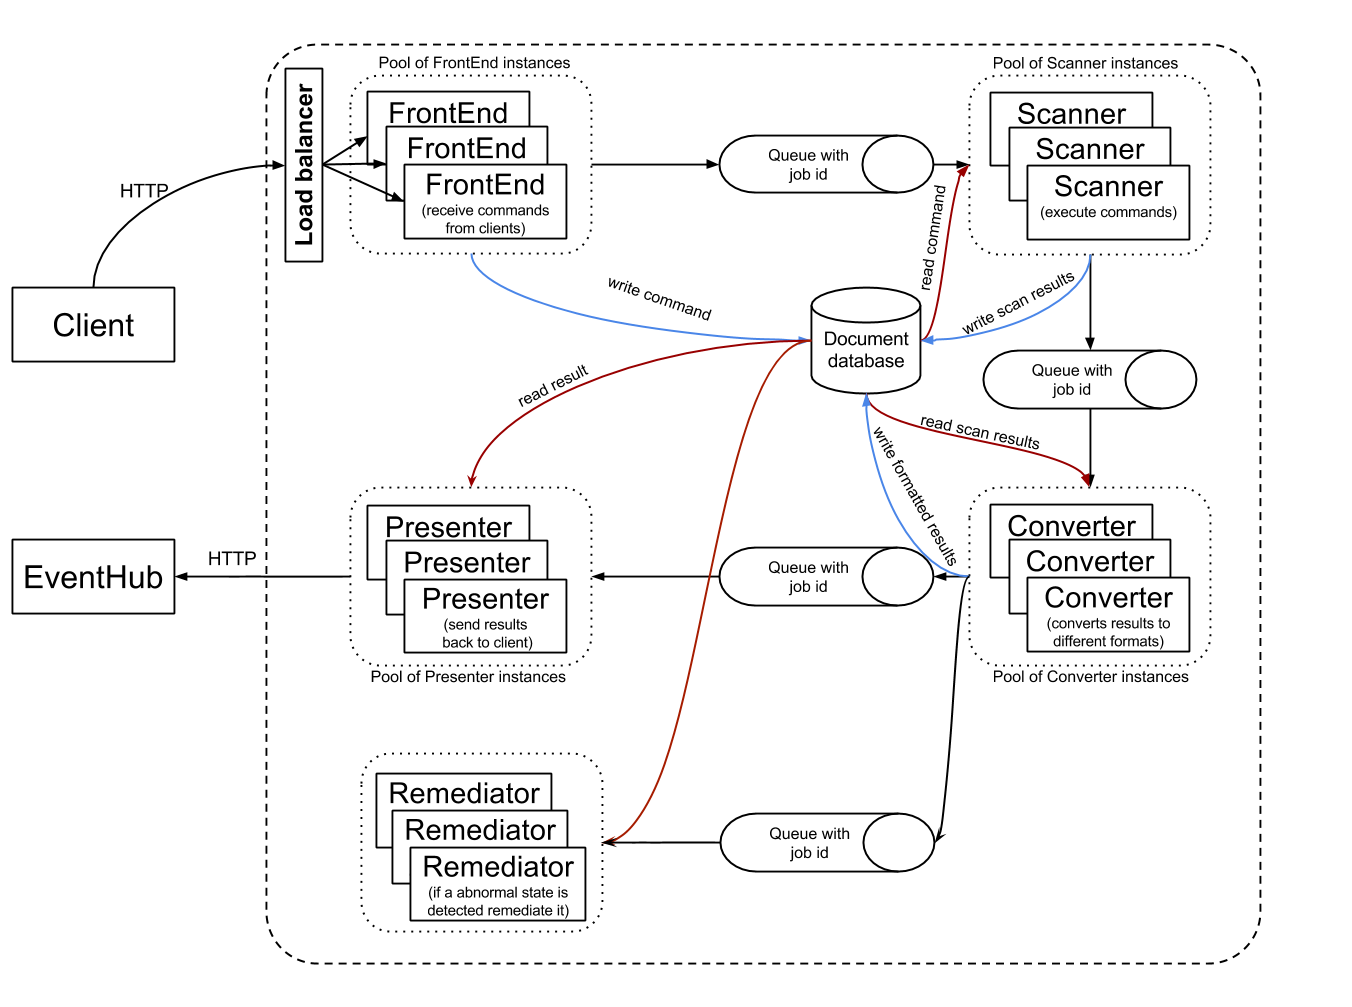
\includegraphics[width=\linewidth]{./img/MonitoringSystemArchitectureRemediation.png}
\caption{Distributed monitoring system architecture}
\label{fig:systemArchitecture}
\end{figure}


\section{Resource allocation for a system with a pipe and filter architecture}
\label{sec:resourceAllocation}
This section focuses on the main challenges of implementing resource allocation without losing benefits like fault tolerance and decoupling between components offered by the pipe and filter architecture. Each of the components can be replicated, but replicas of the same component have no means of organizing, they just take the next job that is available in the queue and execute it, no mechanism for distributing the jobs is in place. Replicas of the same component can consume different amounts of system resources, depending on the type of job they are executing, but because they have no possibility to select the jobs they will execute, they just take the next job from the queue, we cannot predict on which of the replicas the job will be executed. Because of this unpredictability, the task of allocating replicas of components to VMs becomes challenging and different methods have been proposed.

Replicas for the "Scanner" component were used as a case study and the following strategies were considered. Jobs present in the queue were marked as H (high), M (medium), L (low) denoting the CPU usage necessary to complete a job. The following methods were proposed in order to extend the system, taking it one step closer to automatic allocation of resources (components).

\subsection{Method 1: Allows the system to balance work in a natural way and not intervene in job allocation}
\label{subsection:method1}
The first strategy was to let the replicas of the "Scanner" component execute whatever job is available in the queue if they are idle. The main advantages of this strategy is that it does not require any changes to the system, so no extra complexity is added. Fig. \ref{fig:randomDistributionsOfTasks} presents the architecture of the first approach. Another advantage is that components are decoupled as envisioned in the initial architecture Fig. \ref{fig:systemArchitecture}.

The main drawback of this approach is that, because balancing is done by chance, in the worst case, the system could be completely unbalanced, some component executing only high intensive CPU jobs while others executing only low CPU intensive jobs. If more than one "Scanner" replicas run on the same VM, than the chances are even lower for this to happen because, even if some component would be "unlucky" enough to only execute CPU intensive jobs, they would be balanced by other components that execute low intensive CPU jobs from the same machine.

\begin{figure}[ht]
\centering
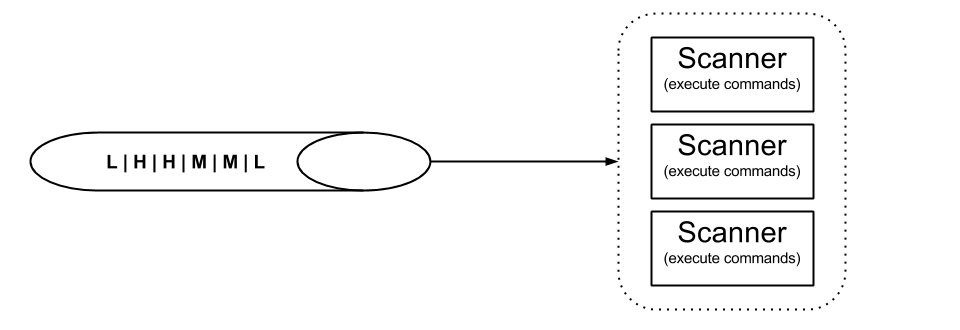
\includegraphics[width=\linewidth]{./img/1_NaturalLoadBalancing.png}
\caption{Random distribution of tasks}
\label{fig:randomDistributionsOfTasks}
\end{figure}

\subsection{Method 2: Assign sizes to jobs and constrain component replicas to execute some type of jobs with a higher priority than others}
\label{subsection:method2}
The second approach Fig. \ref{fig:sizeBaseDistributionOftasks} proposes using some priority scheme inside the "Scanner" component replicas so that we can place "Scanner" replicas on machines that satisfy the required computational needs. For example, if we have a machine with more CPU power, we can allocate "Scanner" replicas that execute CPU intensive jobs. The main advantage of this approach is that we can allocate "Scanner" replicas with different priority schemes to different types of VM's, obtaining a coordinated assignment of component replicas with a knows resource utilization profile. Each replica of the "Scanner" component withdraws messages from the queue, and it makes a decision if it can execute that job or not based on the job type, for example some replicas can only execute CPU intensive jobs (jobs marked with H) while others can execute only low CPU intensive jobs (marked with L). If a replica cannot execute the job, it will just put it back in the front of the queue. Because of this, some messages may spend a very long time in the queue, or even never get executed, if they are always delivered to components that cannot handle them and are put back in front of the queue. Another problem is that the queue is more stressed, because messages are inserted back in the queue if they cannot be executed by a "Scanner" replicas losing the ordering of jobs as well.

\begin{figure}[ht]
\centering
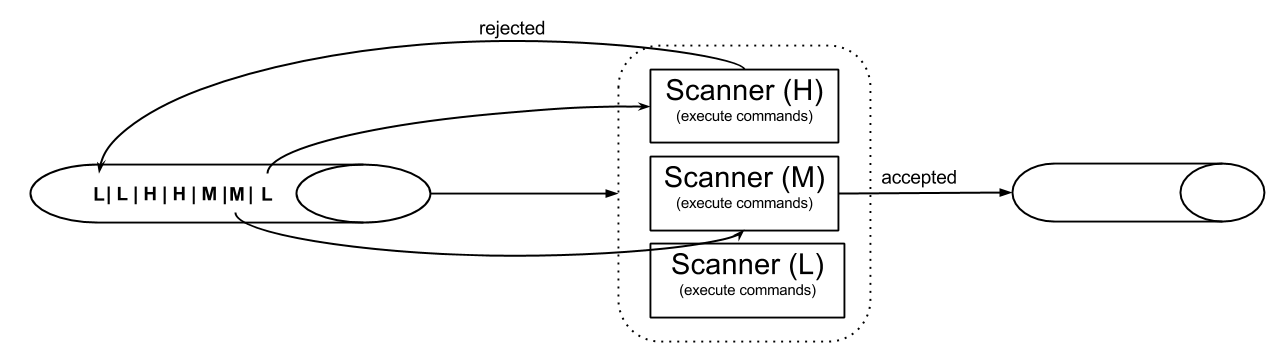
\includegraphics[width=\linewidth]{./img/2_PriorityLoadBalancing.png}
\caption{Size base distribution of tasks}
\label{fig:sizeBaseDistributionOftasks}
\end{figure}


\subsection{Method 3: Create multiple queues depending on the size of the jobs}

The third method Fig. \ref{fig:multipleQueueDistributionOfTasks} uses a messages queue for every type of job, for out example there are three types of jobs (H, M, L), we need three queues and each "Scanner" replica will have a priority scheme that will dictate the priority it gives to each of the message queues. If the "Scanner" replica does not find messages in the queue with the highest priority, it will take messages from another queue with lower priority. The main advantage of this method, compared with the second method \ref{subsection:method2} is that messages are only withdrawn from one queue reducing the load on the queue, and replicas of components don't have to search for jobs, they can just check if there are jobs available on the queues in the order of their priority scheme. Another advantage is that replicas will not be idle or losing time searching for jobs, they will be executing jobs from queues with low priority if there are no jobs in the high priority queue.

The main drawback is that a new message queue is required if we insert a different type of job, and the "Scanner" replicas will be more complex because they need to keep track of all the queues and the priority schemes.

\begin{figure}[ht]
\centering
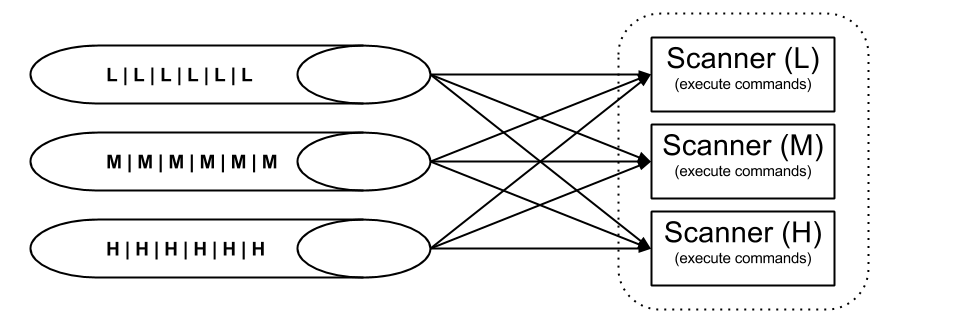
\includegraphics[width=\linewidth]{./img/3_MultipleQueueLoadBalancing.png}
\caption{Multiple queues with multiple size for tasks}
\label{fig:multipleQueueDistributionOfTasks}
\end{figure}

\subsection{Method 4: Use other types of data structure to send the jobs from one component to another}

The forth method Fig. \ref{fig:mapDistributionOfTasks} tries to eliminate all the problems related to job type selection by the "Scanner" replicas by replacing the message queue with a different data structure, in our case a map. In this approach, each "Scanner" replica can inspect all the jobs that can be executed and pick the one best suiting their capabilities.

Although this approach eliminates most of the disadvantages we had when using message queues, it eliminates most of the guarantees that were offered by them as well. Job order is not preserved, the map is a shared by all replicas and operations to it must be serialized to avoid conflicts, or a conflict resolution mechanism should be implemented. Some mechanism for acknowledgment of jobs completion must be implemented in order to avoid losing jobs when components fail.

\begin{figure}[ht]
\centering
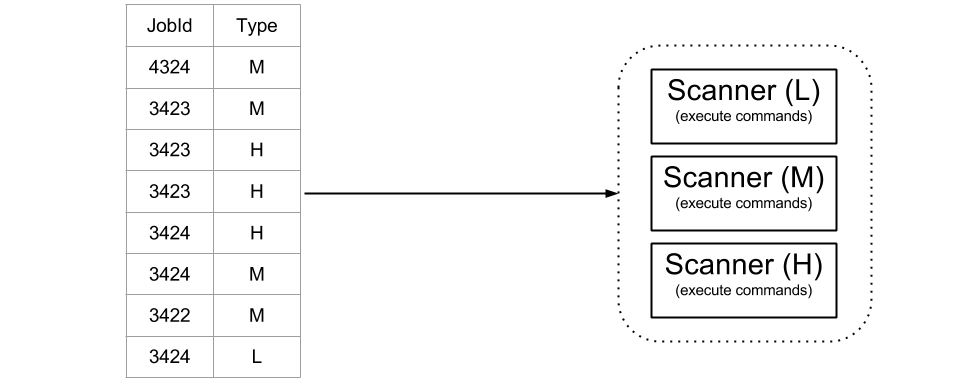
\includegraphics[width=\linewidth]{./img/4_MapOrOtherDataStructureLoadBalancing.png}
\caption{Map with multiple size tasks.}
\label{fig:mapDistributionOfTasks}
\end{figure}

\subsection{Choosing one method}
One of the assumption made at the beginning of this section was that we can determine in advance the CPU usage for jobs, but this can prove to be very difficult in practice because there are more than 3 types of jobs and their CPU usage depends on other factors like network speed and the speed of response for a particular host, network configuration, etc.

As a starting point we chose the method presented in \ref{subsection:method2} because it does not break any of the properties of the system, it can be later extended to any of the more advanced methods and in practice we observed that "Scanner" replicas tend to balanced themselves naturally, without any intervention.
\section{Gathering performance metrics}
Although the system is very flexible and allows replication of components, it does not contain any component that is able to evaluate it's state and make decisions regarding allocation and release of resources consequently scaling must be done manually. Manual scaling the system can become a complex problem because each component has different resource requirements and even the same component can use more or less of a resource, depending on the job that it must execute. Monitoring the system manually and scaling it quickly become unmanageable and an automated way to do the scaling is desirable. 

In order to scale the system automatically, key performance metrics must be gathered and analyzed. 

Some of the basic performance parameters that can be gathered for a component are CPU, memory and network usage. Knowing the resource utilization of one component allows us to take decisions regarding deployment of that component. For example we can have 2 component, one with high CPU usage and one with high network usage, it would be wise to combine replicas of those components on the same VM or to allocate the ones that require high CPU usage to VM's with powerful CPU. By having this insight on component resource utilization we are able to take those decisions and to use the resources that we have in an efficient way. But resource utilization for components can vary with time, so a static scheme is not very useful, because it becomes outdated in a short period of time. Conterminous monitoring the components and taking actions on fresh performance metrics is crucial in guaranteeing optimal allocation strategies.

\subsection{Monitoring CPU}
A first step would be to monitor the CPU usage in order to find a rough approximation of how much computing power does a component need. The main challenge here is to find tools that are able to monitor short lived processed (under 1 second) and to report with high accuracy the CPU usage because sometimes components can use very little CPU. Four tools / methods of gathering CPU usage statistics were reviewed:  
\begin{itemize}
	\item Using a class from the Java library called "ManagementFactory" is a good way to measure the Java program, the main drawback is that Nmap is an external program and it cannot be monitored by this library.
	\item Sigar library for Java can be used to monitor arbitrary process id's (PIDs), but the problem is that we first have to start the component, obtain it's PID and only after we can start monitoring it with "Sigar" library, the main problem is that we might lose the CPU usage at the start of the process which can be introduce high error rates.
	\item pidstat and top have the same drawbacks. they miss the CPu usage for the process if it is very short lived, they miss the CPU usage of the process right before it ends, but they are better alternatives than the tools mentioned before because they can monitor processes from the moment they are crated, not missing the CPU usage from the start of the process.
	\item atop can monitor processes from the moment they are crated and capture the CPu usage of the process right before it terminated. Because it is able to capture the CPU usage at the start and at the end of the lifetime of a process, it provides very accurate results introducing small overhead on the system. The only drawback that was found is related to the root privileges that are needed in order to run this tool.
\end{itemize}
 
The tool atop was chosen to measure CPU usage because of it's high accuracy and low overhead. In the first implementation "atop" was called at the begging of each new job for each component, but this approach had many drawbacks: because it took some time to start atop, some CPU usage might be lost, and it required launching atop for each job and for each component making it consume considerable system resources. The second approach was to use launch "atop" from an external script, parse it's results and store them in a log file. Each component that is interested in it's or others component CPU usage can just parse the log and search after the PID of interest between a time intervals. This second approach was much better because it allowed using only 1 atop instance to gather CPU usage statistics for all running processes on a system, and each component that was interested in it's CPU usage could have just parsed the log file. Another advantage was that it decoupled the monitoring activities from the components that were monitored. The architecture for the second approach is presented in Fig. \ref{fig:monitoringArchitecture}, the log document is read from the bottom upwards, because the chances are that the monitoring results will be closer to the bottom than to the top.

\begin{figure}[ht]
\centering
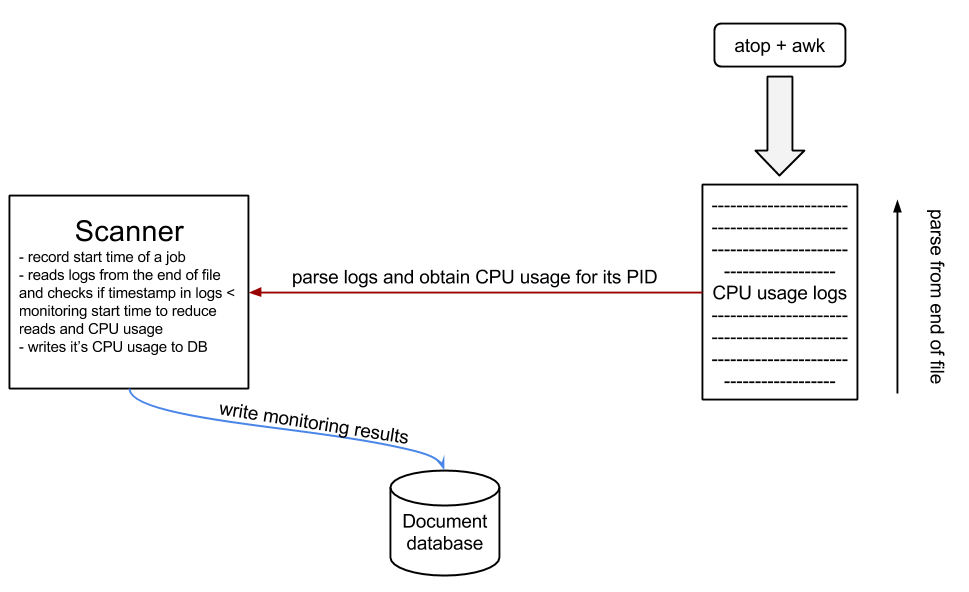
\includegraphics[width=\linewidth]{./img/MonitoringCPUMechanism.png}
\caption{Distributed monitoring system architecture}
\label{fig:monitoringArchitecture}
\end{figure}

Fig. \ref{fig:monitoringArchitectureExtended}  presents an architecture that is even more decoupled than the one that was implemented, the parsing is done in a different component "Monitor" and the components only need to save the beginning and the end time for a job they executed, the parsing of the monitoring data would be done by the "Monitor" component. This architecture ads more flexibility, because the Monitor component can be on the same machine to minimize network traffic (otherwise the log would have to be transfered to the machine that holds the "Monitor" component) or on a different machine.


\begin{figure}[ht]
\centering
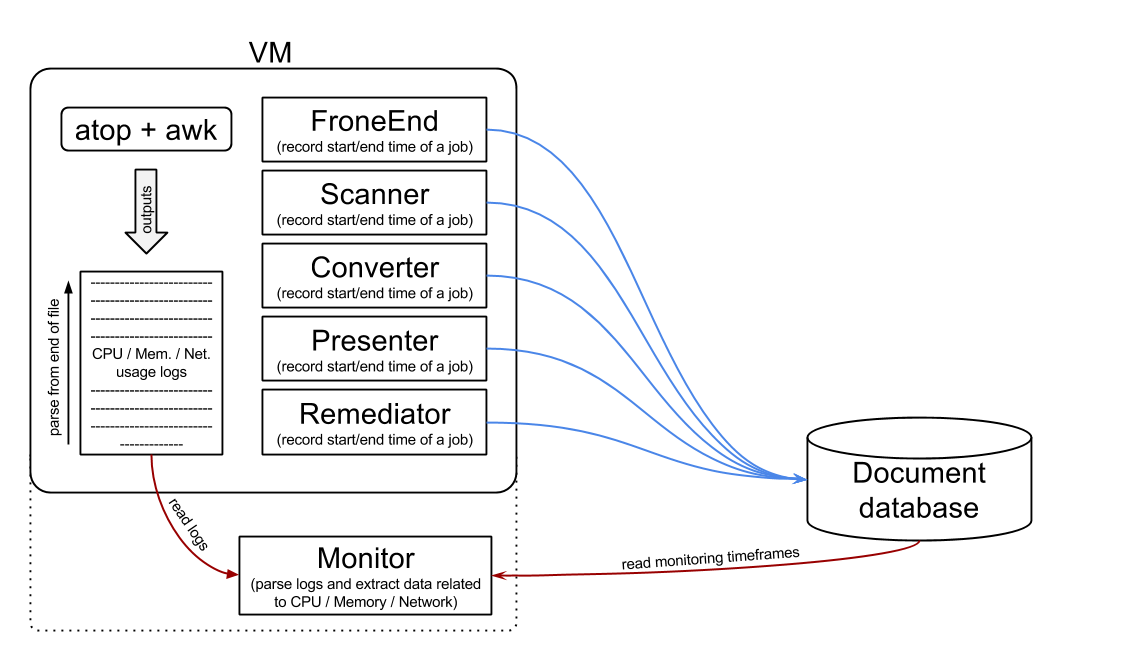
\includegraphics[width=\linewidth]{./img/MonitoringCPUMechanismExtended.png}
\caption{Distributed monitoring system architecture}
\label{fig:monitoringArchitectureExtended}
\end{figure}

\section*{Conclusions}
The paper presents extensions for a system that is built on a pipe and filter architecture. Four possible architectures Fig. \ref{fig:randomDistributionsOfTasks} \ref{fig:sizeBaseDistributionOftasks} \ref{fig:multipleQueueDistributionOfTasks} \ref{fig:mapDistributionOfTasks} were suggested, each one with its advantages and disadvantages. Several ways of monitoring performance were tested and a monitoring architecture was built around "atop" software tool. 

The work from this paper bring to system from \cite{IrimieAndPetcu} one step closer to the main objective of dynamic allocation of components on virtual machines. Constant change in resource utilization of each component replica must be taken into account in order to predict the VM where to allocate a component replica and continuous performance monitoring must be implemented in order to record the change in resource utilization of each component replica. The next step is to build a component that is able to use the performance metrics gathered and make allocation plans taking into account the constraints of the architecture of the system.

\section*{Acknowledgements}

The work conducted in this report was supported by EC FP7 project Secure Provisioning of Cloud Services based on SLA management, SPECS (Grant Agreement no. 610795) and Competitive Multidisciplinary Doctoral Research in Europe (CDocMD) POSDRU/187/1.5/S/155559 project. The author would like to thank members of the Department of Computing from Imperial College London for their advice and guidance.

\bibliographystyle{./class/IEEEtran}
\bibliography{./bib/report.bib}

\end{document}
